\documentclass[9pt]{beamer}
\usetheme{Warsaw}
\usepackage[utf8]{inputenc}
\usepackage[english]{babel}
\usepackage{amsmath}
\usepackage{amsfonts}
\usepackage{amssymb}
\usepackage{graphicx}
\usepackage{tikz}
\usetikzlibrary{
	arrows,
	automata,
        shadings,
        shadows,
        shapes,
}

\usepackage{fontspec}
\newfontfamily\cjkfont{Noto Sans CJK SC} % Or any appropriate font you have

\input{global_color_scheme.tex}
\input{tikz_process_steps/contsts.tex}

\author{leviathanch | chipforge | foshardware \ (Lanceville Technology)}
\title{Breaking the microchip monopoly}
\setbeamercovered{transparent} 
\setbeamertemplate{navigation symbols}{} 
\logo{lsa.png} 
%\institute{} 
%\date{} 
\subject{A free semiconductor manufacturing standard}
\begin{document}

%\begin{frame}
%\tableofcontents
%\end{frame}

\section[Standard Cells]{}
\begin{frame}{Standard Cells}
\end{frame}

\section[Silicon Compiler]{}
\begin{frame}{Open Source Tools}
	\begin{itemize}
        \setlength\itemsep{1em}
		\item yosys
		\item graywolf
		\item qrouter
		\item several FPGA routers
	\end{itemize}
\end{frame}

\begin{frame}{graywolf}
	\begin{itemize}
        \setlength\itemsep{1em}
		\item Originates in Academia: TimberWolf
		\item Simulated annealing
	        \begin{itemize}
		    \item Meta heuristic that is useful not only for placement
	        \end{itemize}
		\item Inline syscalls
	        \begin{itemize}
		    \item This is just a bad idea
	        \end{itemize}
	\end{itemize}
\end{frame}

\begin{frame}{qrouter}
	\begin{itemize}
        \setlength\itemsep{1em}
		\item Started in 2011 by Tim Edwards 
		\item Widely used for FPGA
	        \begin{itemize}
		    \item Not ready for silicon
	        \end{itemize}
		\item Sequential routing
	        \begin{itemize}
		    \item Parallelism not in scope
	        \end{itemize}
		\item Difficult to prove formal correctness
	        \begin{itemize}
		    \item Prove that C implementation of Rip-up and Re-route is correct
	        \end{itemize}
	\end{itemize}
\end{frame}

\begin{frame}{Productive Tools}
	\begin{itemize}
        \setlength\itemsep{1em}
		\item Different tool sets like BonnRoute, Cadence Suite, Alliance tools, etc.
		\item Similar capabilities with respect to silicon
		\item Just throw man-power at VLSI --- what is automation?
	\end{itemize}
\end{frame}

{ 
\setbeamertemplate{background canvas}{\includegraphics[height=\paperheight,width=\paperwidth]{images/VLSI01.jpg}} 
\begin{frame}[plain] 
\end{frame} 
} 

\begin{frame}{Routing: State of the Art}
	\begin{itemize}
        \setlength\itemsep{1em}
		\item Place components for a large chip
		\item Route wires roughly along a chessboard for a large chip
		\item Route detailed tracks and vias for a large chip
		\item Formal correctness: Rip-up and Re-route
		\item Formal style: Sequential/Imperative code
	\end{itemize}
\end{frame}

\begin{frame}{Routing: Proposed}
	\begin{itemize}
        \setlength\itemsep{1em}
		\item Decomposition for a large chip
		\item Place components and route for small chips in parallel
		\item Place abstract gates and route recursively
		\item Formal correctness: Reduction from SMT
		\item Formal style: Parallel/Declarative code
	\end{itemize}
\end{frame}

\begin{frame}{Divide and Conquer}
	    \textbf{Academia + Industry:}
	    \begin{itemize}
		\item Placement and Routing are different problems
		\item All components map to the same problem
	    \end{itemize}
	    \textbf{LibreSilicon:}
	    \begin{itemize}
		\item Placement and Routing are the same problem
		\item Different components map to different problems
	    \end{itemize}
\end{frame}

\begin{frame}{Routing Hierarchy}
	    \textbf{Academia + Industry:}
	    \begin{itemize}
		\item Geographical partitioning of a wafer $\rightarrow$ \textit{cut tree}
		\item Based on preceeding placement steps
	    \end{itemize}
	    \textbf{LibreSilicon:}
	    \begin{itemize}
		\item Modular chip development $\rightarrow$ \textit{subcell hierarchy}
		\item Subcells carry implicit and explicit subcells
	    \end{itemize}
\end{frame}

\begin{frame}{Frontier: Parallelism}
	\begin{itemize}
        \setlength\itemsep{1em}
		\item BonnRoute: concurrency + shared memory model
		\item qrouter: none 
		\item lsc: map + reduce
	\end{itemize}
\end{frame}

\begin{frame}{Subcell hierarchies}
	\begin{itemize}
        \setlength\itemsep{1em}
		\item Explicit subcell hierarchies through high modularization
		\item Implicit subcell hierarchies through exlining
		\item Preserve hierarchy in compiler interfaces
	\end{itemize}
\end{frame}

\begin{frame}{High modularization}
        \begin{figure}
        \centering
        \includegraphics[scale=0.32]{images/SystemBus.png}
        \end{figure}
\end{frame}

\begin{frame}{Exlining}
	\begin{itemize}
        \setlength\itemsep{1em}
		\item Proof of concept: picorv
	\end{itemize}
\end{frame}

\begin{frame}{Unconstrained Small Unified Silicon Problem}
	\begin{itemize}
        \setlength\itemsep{1em}
		\item Components and nets $\rightarrow$ \textit{rectilinear geometries}
		\item Components do not overlap
		\item Nets overlap with their pins on components
	\end{itemize}
\end{frame}

\begin{frame}{Minimizing Goals}
	\begin{itemize}
        \setlength\itemsep{1em}
		\item Layout area
		\item Maximum wire length 
		\item Via count
		\item Crossing number (computational)
		\item Wire jogs (minor)
	\end{itemize}
\end{frame}

\begin{frame}{Defining rectangular components}
	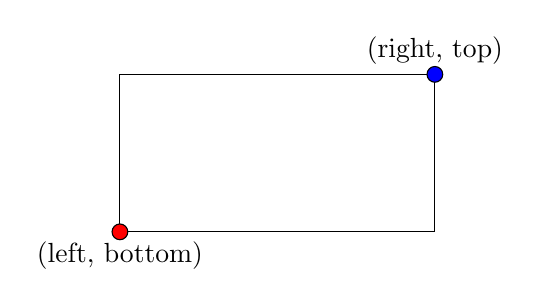
\begin{tikzpicture}
            \draw (0,-8) rectangle (4,-6);
            \draw[fill=red]  (0,-8) circle (0.1);
            \draw[fill=blue] (4,-6) circle (0.1);
            \node at (0,-8.3) {(left, bottom)};
            \node at (4,-5.7) {(right, top)};
	\end{tikzpicture}
\end{frame}

\begin{frame}{Overlaps}
	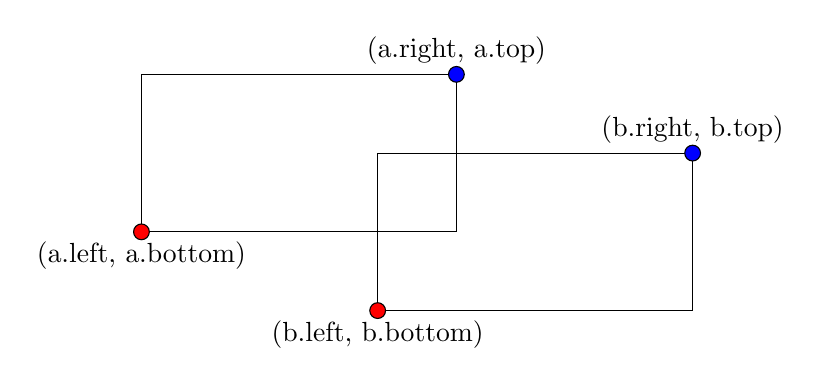
\begin{tikzpicture}
            \draw (0,-8) rectangle (4,-6);
            \draw[fill=red]  (0,-8) circle (0.1);
            \draw[fill=blue] (4,-6) circle (0.1);
            \node at (0,-8.3) {(a.left, a.bottom)};
            \node at (4,-5.7) {(a.right, a.top)};
            
            \draw (3,-9) rectangle (7,-7);
            \draw[fill=red]  (3,-9) circle (0.1);
            \draw[fill=blue] (7,-7) circle (0.1);
            \node at (3,-9.3) {(b.left, b.bottom)};
            \node at (7,-6.7) {(b.right, b.top)};
	\end{tikzpicture}
\end{frame}

\begin{frame}{Reduction from SMT}
        b.left > a.right
    $\parallel$ a.bottom > b.top
\end{frame}

\begin{frame}{Combining in the LSC Semigroup}
    overlap + net connect + another constraint
\end{frame}

\begin{frame}{Just stay here}
    non-critical EXP
\end{frame}

\begin{frame}{Maximize yield}
    Compiler versus. process
\end{frame}


\section[Process]{}

\begin{frame}{Features}
	\begin{itemize}
        \setlength\itemsep{1em}
		\item MOSFETs
		\item LDMOSFETs (High voltage) 
		\item BJTs
		\item Zener polysilicon diodes
		\item SONOS flash cells
		\item Polysilicon resistors
		\item Metal caps
	\end{itemize}
\end{frame}

\begin{frame}{Cross section}
\begin{center}
	\begin{tikzpicture}[node distance = 3cm, auto, thick,scale=0.2, every node/.style={transform shape}]
		\input{tikz_process_steps/glass.a.tex}
		\node at (5,-0.5) {\textbf{\huge{PMOS}}};
		\node at (13,-0.5) {\textbf{\huge{NMOS}}};
		\node at (22,-0.5) {\textbf{\huge{SONOS flash cell (PMOS)}}};
		\node at (30,-0.5) {\textbf{\huge{NPN BJT}}};
		\node at (38,-0.5) {\textbf{\huge{PNP BJT}}};
		\node at (46,-0.5) {\textbf{\huge{Polysilicon diode}}};
		\node at (52,-0.5) {\textbf{\huge{Polyresistor}}};
	\end{tikzpicture}
\end{center}
\end{frame}

\begin{frame}{PearlRiver \cjkfont(珠江芯片一号)}
\begin{center}
\includegraphics[width=1.0\textwidth]{images/Screenshot_20181216_204924.png}
\end{center}
\end{frame}

\begin{frame}{PearlRiver \cjkfont(珠江芯片一号)}
	\textbf{Fulfills following functions:}
	\begin{itemize}
		\item Debugging
		\item Calibration of new equipment to LibreSilicon
		\item Research of new features
		\item Syncing process features between fabs
	\end{itemize}
\end{frame}

\begin{frame}{Photomask}
\begin{center}
\includegraphics[width=0.5\textwidth]{images/20181207_113845_Burst01.jpg}
\end{center}
\end{frame}

\begin{frame}{Photomask}
	\begin{itemize}
		\item Is stepper/aligner brand specific
		\item ASML stepper masks contain 4 layers each
		\item The NFF stepper has a reduction value of 5:1
		\item A 5 micron gate on the mask is 1 micron on the wafer
	\end{itemize}
\end{frame}

\begin{frame}{Photo resist}
\begin{center}
\includegraphics[width=0.4\textwidth]{images/20181128_154907.jpg}
\includegraphics[width=0.4\textwidth]{images/20181128_154911.jpg}
\end{center}
\end{frame}

\begin{frame}{Photo resist}
	\textbf{Two types of photo resist:}
	\begin{itemize}
		\item FH 6400L (implantation)
		\item HPR 504 (normal etch)
	\end{itemize}

	\textbf{Factors to consider:}
	\begin{itemize}
		\item Thickness of FH 6400L and implantation energy are interlinked
		\item Thickness of HPR 504 and etching time are interlinked (selectivity)
	\end{itemize}
\end{frame}

\begin{frame}{After exposure}
\begin{center}
\includegraphics[width=0.4\textwidth]{images/20181210_125830_Burst01.jpg}
\includegraphics[width=0.4\textwidth]{images/20181210_125845.jpg}
\end{center}
\end{frame}

\begin{frame}{Alignment}
\begin{center}
\includegraphics[width=0.4\textwidth]{images/20181211_125918.jpg}
\includegraphics[width=0.4\textwidth]{images/20181211_161801_Burst01.jpg}
\end{center}
\end{frame}

\end{document}
